\documentclass{article}
\usepackage[utf8]{inputenc}
\usepackage[a4paper, total={5.5in, 9in}]{geometry}
\usepackage{biblatex}
\usepackage{todonotes}
\usepackage{amsmath}
\usepackage{titlesec}
\usepackage[T1]{fontenc}
\usepackage{nameref}

% TODO: Tren og evaluer standard 300, kompleks 300, attention bot
% skriv rapport
% Kok fra den andre rapportgreia

% Capitalize sections
\titleformat{\section}
  {\normalfont\fontsize{11pt}{12pt}\selectfont\bfseries}{\thesection}{1em}{\MakeUppercase}

\renewcommand\abstractname{ABSTRACT}
\renewenvironment{abstract}
 {\small
  \begin{center}
  \bfseries \abstractname\vspace{0em}
  \end{center}
  \list{}{
    \setlength{\leftmargin}{12.5mm}%
    \setlength{\rightmargin}{\leftmargin}%
  }
  \item\relax}
 {\endlist}

 \renewcommand{\arraystretch}{1.2}
 
\addbibresource{references.bib}

\title{\textbf{Language Agnostic Generative Chatbot using Personal Chat log
Data}}
\author{Torjus Iveland \and Vegar Andreas Bergum}
\date{}

\begin{document}

\maketitle
\centerline{\textit{TDT4310 - Intelligent Text Analytics and Language
Understanding}}
\centerline{\textit{Norwegian University of Science and Technology}}
\centerline{\textit{Trondheim, Norway --- April 2019}}
\vspace{6mm} % Space above abstract

\begin{abstract}

This report explores the state of Norwegian chatbot systems with
the aim of verifying that conventional English chatbot creation techniques
also can be used to create chatbots which converse in Norwegian. There are
multiple challenges with Norwegian chatbots, due to the syntactic structure
of the language as well as the lack of available training data.

\paragraph{}
We present an implementation of a generic-domain chatbot system using a simple
sequence-to-sequence model, a kind of model which primarily is applied to
neural machine translation but which also has proven effective for chatbot
systems. We believe our results illustrate that neural machine translation
techniques indeed can be applied to create chatbots in both Norwegian as
well as English, as long as enough training data of a sufficiently high
quality is available. However, we stress that in many cases such training
data in Norwegian can be hard to obtain.
\end{abstract}
\vspace{3mm}

\section*{Introduction}
A chatbot is a computer system which can interact with an user through natural
language. Because humans tend to prefer more human-like interfaces, chatbots can
be very useful in applications
such as customer support, education, and personal productivity systems like
Google Assistant.  This project concerns such chatbots which converse
specifically using the Norwegian language.

\paragraph{}
Most research on chatbot systems concerns chatbots which converse in English.
However, Norwegian has a syntactic structure which differs from that of
English. Therefore, it is not guaranteed that this research automatically
applies to Norwegian chatbots as well. Additionally, further problems arise
from the fact that training data in Norwegian is not as abundant as for
English.

\paragraph{}
In this project, we explore Norwegian chatbots, with the goal of verifying that
conventional chatbot-creation techniques also can function adequately in
Norwegian. We especially want to verify that deep learning techniques such as
sequence-to-sequence models \cite{Cho2014} can be used to create
general-purpose Norwegian chatbots. Such models are usually used for machine
translation, but they have also proven effective in the field of chatbots. The
main objective of this project is therefore to implement a simple Norwegian
chatbot using a sequence-to-sequence model, which for example could be used as
a small talk module in another mode domain-specific chatbot.

\paragraph{}
We differ between retrieval-based and generative chatbots. A retrieval-based
system usually map an user input to a predefined intent, and then retrieve an
answer from a set of answers belonging to the detected intent. A generative
system does not rely on such predefined sets of answers.  Instead, they are
able to automatically generate an answer to the provided query. In this
project, we restrict ourselves to the latter kind of model. We also restrict
ourselves to an user-initiative only model, which means that the chatbot simply
responds with an answer to each user query.

\if
- Something about how we want to structure the rest of the report.  
- Fix that goal, motivation, question and hypothesis are not clear.  
- Attention \cite{Bahdanau2015}, BERT and similar when we hopefully begin using it.
\fi


\section*{Method}
% I dette kapitlet skal du skrive om hvordan du har gått frem metodisk, og vise
% hvordan valg av design og metode egner seg til å svare på problemstillingen
% din.  Kapitlet må kunne gi svar på disse spørsmålene: Hvordan samlet du inn
% datamaterialet?  Hvordan behandlet du dataene du samlet inn?  Hvorfor valgte
% du disse metodene?  Hva er styrkene og svakehetene ved disse metodene?  Du
% skal også si noe om hvorfor du har gjort din undersøkelse på den måten du
% gjorde – og da peke på styrker og svakheter. I tillegg skal du drøfte etiske
% aspekter ved prosjektet. På den måten viser du at du har kommet frem til
% resultatene på en pålitelig og troverdig måte, men også at du er reflektert
% og kritisk overfor arbeidet du har gjort.  Husk også at du her, slik som i
% teorikapitlet, bare skal skrive om det metodiske som er relevant for din
% studie.
\if
 - Prøvd ut pre-existing modeller med forskjellige datasett
    - engelsk datasett som vi vet er av god kvalitet
    - forskjellige attention-modeller
 - Sammenlignet egne modeller og eget datasett mot dette
 - Ressursbegrensning (datakraft og tid) har begrenset omfanget på evaluering
 av forskjellige modeller
\fi

This project's main goal was to explore the possibility of generative chatbots
in Norwegian. One of the prerequisites for a language specific language
generation system to work is data. The language generation method is highly
dependant on the amount and quality of data available. The method of choice was
the sequence-to-sequence model proposed by Cho et al. in their paper \cite{Cho2014}.

\paragraph{}
Sequence-to-sequence models have proven to be an excellent baseline for
chatbots \cite{Vinyals2015}. When considering a user-initiative only model the
task of a generative chatbot system can be reduced to mapping introductory
utterances to a target utterance.  Models with a sufficiently large corpus for
example-based `translation' had been shown to produce promising results in the
given corpus language \cite{Ezquerra2018}. Although these bots are not able
apply any logic to their answers, they are able to mimic natural human
language.

\paragraph{}
The architecture is built using Google's Machine Learning framework TensorFlow
as a backend with Keras as a high level wrapper. The architecture looks at a
model using Long Short Term Memory (LSTM) nodes with word-level context and a
three-dimensional sequence embedding. This architecture can be further
developed using a word-level embedding such as \textit{Word2Vec}
\cite{word2vec} and sequence-level context like the Bahdanau Attention mechanism
\cite{Bahdanau2015}.
\todo{Rewrite paragraph slightly. Also add more information about why
we believe this will illustrate the effectiveness of Norwegian chatbots.}
\todo{Planen er å vise at norske chatbots går an, sammenligne flere
forskjellige}

\section*{Data}
Norwegian chatbot training data is not readily available, but relevant corpora
still exist.  For example, multiple spoken language corpora are available
through the CLARINO project \cite{clarino-about}. Examples of CLARINO
corpora which might prove useful for a chatbot project are the Big Brother
corpus \cite{clarino-bb} and NoTa-Oslo \cite{clarino-nota}, which both provide
spoken language annotations for he Norwegian language. However, both these
corpora have quite restrictive licenses and are only accessible online for
privacy reasons. Thus, the CLARINO corpora are not well suited for our chatbot
usage.

\paragraph{}
Another possible data source is to use exports of personal chatbot data from
various online platforms, For example, Facebook allows users to export their
private Messenger chat data. If all parties involved in a conversation consent,
such data can be used to train a chatbot. An average Facebook user will quite
easily be able to generate several tens of thousands of utterances over the
course of a few years. More avid users of the platform can have chat logs
containing several hundred thousands or even millions of messages. This project
combines the utterances of two Facebook users, ending in a corpus with more
than 110,000 utterance pairs.
\todo{vil vi ha med noe om challenges mtp at svar kan variere veldig fra person
til person? svar: ja}
\todo{want to use norwegian chat data to verify...}

\paragraph{}
In addition to using personal Facebook Messenger data, the Cornell Movie
Dialogs Corpus \cite{cornell-corpus} has been used for model evaluation. The
Cornell corpus consists of several hundreds of thousands utterances from movie
scripts that are freely available. This corpus is frequently highlighted in
chatbot models as a high quality data set.
\todo{difficulties with chatbot data. want to check if it is possible
to use real }
\todo{used this dataset for cross-checking}

\section*{Implementation}
Chatbots which utilise deep learning are usually based on sequence to sequence
models. A sequence to sequence model is a type of architecture where there is
an encoder RNN and a decoder RNN. For usages such as machine translation and
chatbots, the idea is that we feed the encoder RNN input words one at a time,
which eventually results in an output vector describing the input sentence.
This output vector is sometimes referred to as a thought vector, as it stores
the systems understanding of the input. For machine translation, we would feed
the encoder RNN the sentence to be translated, and for chatbots, the encoder
RNN would accept the input sentence which should be responded to. The decoder
RNN is trained to take thought vectors from the encoder and output tokens
one by one until an end of sequence token is outputted. Since the decoder
network is dependent on the output of the encoder network, both networks are
trained together. This simple model has proven very effective for neural
machine translation and other tasks as well. An early description of this
architecture is available in \cite{Cho2014}.

\paragraph{}
The rest of this section is dedicated to describing the architecture of
this project. We first describe the preprocessing phase, then the model which
is being used, and finally the inference phase, in which the responses to user
utterances are actually generated.

\subsection*{Preprocessing}
Before the data is forwarded to the model, it needs to be preprocessed. The
preprocessing phase in this project consists of a number of steps. We use
data from Facebook Messenger to train our chatbot. To split the data into
input and target data sets, we simply treat each utterance as the input to
the next utterance - that is, each utterance is the response to the previous.

\paragraph{}
First, text is normalized by removing all punctuation from the text. Newlines
are replaced with spaces, and all text is converted to lower-case. Ideally,
the bot should output grammatically correct text, but this requires a
significantly more complex model. We use the Norwegian NLTK tokenizer to split
the text into words. Lastly, each utterance is wrapped in a special start and
end token, which indicates to the model when it should stop generating text
during the inference phase.

\paragraph{}
The preprocessing system also performs filtering on which utterances should
and should not be used. For example, the system can be configured to only
use responses from a specific person, to give the chatbot a more distinct
personality. Additionally, the system can removes self-replies, so that
only discourse between two different persons is considered.

\paragraph{}
The maximum length of an input or target utterance is capped at 20 tokens.
This is required to reduce the size of the input matrices for the model, due
to limited available computational power. However, an analysis of the dataset
shows that only about 4\% of the utterances are above this limit. Similarly,
we limit the number of words which may appear in the input and target data.
This vocabulary size only includes the most common 3000 words. In accordance
with Zipf's law, 3000 words accounts for slightly under 80\% of the total
vocabulary. While this might reduce the quality of the output due to certain
parts of the output sentences being omitted, it is crucial that the size of
the input vectors is minimized.

\subsection*{Feature extraction}
\todo{Is feature extraction the correct term?}
The preprocessing system also provides a way of encoding utterances as
vectors, a process known as word embedding. This is done by simply
encoding each token as an unique number, with additional logic for handling
unknown tokens. Note that this is a very simple embedding technique, and
therefore future work might include exploring alternative embedding techniques
such as \emph{Word2Vec} \cite{word2vec} or \emph{BERT} \cite{bert2018}.
We now provide a high-level conceptual overview of the feature extraction
process used in this project.

\paragraph{}
With a corpus $D = \{\text{``How are you doing?''}\}$ containing utterances, 
a vocabulary $\vec{V}$ containing all distinct words in the corpus is
constructed. This is used to build a mapping where each token is mapped to
its corresponding index in the vocabulary vector $\vec{V}$. This mapping is
then used to encode utterances as vectors. Table 1 illustrates
%WATCHOUTWATCHOUTWATCHOUTWATCHOUTWATCHOUTWATCHOUTWATCHOUT
this mapping. Note that there are three special tokens representing beginning
of sequence, padding and end of sequence.
\todo{Refer to more equations and fix broken table reference.}

\begin{equation}
   \vec{V} = [ \textrm{<BOS>},\, \textrm{<PAD>},\, \textrm{``how''},\,
               \textrm{``are''},\, \textrm{``you''},\, \textrm{``doing''},\,
               \textrm{<EOS>}]
 \end{equation}

\begin{table}[hbt]
  \begin{center}
    \begin{tabular}{c|c|c|c|c|c|c|c}
      \textbf{Index} & 0 & 1 & 2 & 3 & 4 & 5 & 6 \\
      \hline
      \textbf{Token} & <PAD> & <BOS> & how & are & you & doing & <EOS> \\
    \end{tabular}
  \end{center}
  \label{tab:tok2num}
  \caption{Token to number mapping}
\end{table}

\paragraph{}
In order to maintain a fixed dimensionality of our sequence embeddings there
needs to be predefined sequence length. In this example this is set to 5. If a
sequence is shorter than this, the rest of the sequence matrix is filled with
padding tokens. Using the vocabulary above, the word ``how'' is mapped to the
word vector $\vec{v}_2$.

\begin{equation}
  \vec{v}_2 = [0, 0, 1, 0, 0, 0, 0] \quad {\leftrightarrow} \quad \textrm{``how''}
\end{equation}

\paragraph{}
Using these word vectors, a matrix of one-hot encoded row vectors can be
constructed by a vector of row vectors. The matrix $d_0$ is the embedding of
the utterance sequence in the initial dataset $D$.  

\begin{equation}
  d_{0} = 
    \begin{bmatrix}
      0 & 1 & 0 & 0 & 0 & 0 & 0\\
      0 & 0 & 1 & 0 & 0 & 0 & 0\\
      0 & 0 & 0 & 1 & 0 & 0 & 0\\
      0 & 0 & 0 & 0 & 1 & 0 & 0\\
      0 & 0 & 0 & 0 & 0 & 1 & 0\\
      1 & 0 & 0 & 0 & 0 & 0 & 0\\
      0 & 0 & 0 & 0 & 0 & 0 & 1\\
    \end{bmatrix}
\end{equation}

\paragraph{}
Equation \ref{eq:seq-out} show the exact sequence represented by $d_0$. Notice
that its length is 5, excluding the beginning- and end of sequence tokens.

\begin{equation} \label{eq:seq-out}
  [ \textrm{<BOS>},\, \textrm{``How''},\, \textrm{``are''},\, \textrm{``you''},\,
    \textrm{``doing''},\, \textrm{<PAD>},\, \textrm{<EOS>} ]
\end{equation}

\paragraph{}
This sequence embedding is used to extract the necessary features needed to
make a statistical prediction of the next token in an output sequence, given an
input sequence. The extracted features are the context of the token's
occurrences.

\subsection*{Model}
This project utilises a fairly standard sequence-to-sequence model implemented
using Keras, which is illustrated in figure \ref{fig:keras-model}. The encoder
conists of an input layer, another layer with dropout and an LSTM layer which
feeds into the decoder. The decoder is strictured similarly, consisting of an
input layer, a dropout layer, a decoder dropout layer and a dense layer as the
last layer of the model.

\begin{center}
  \begin{figure}[hbt]
    \centering
    \makebox[\linewidth][c]
      {
        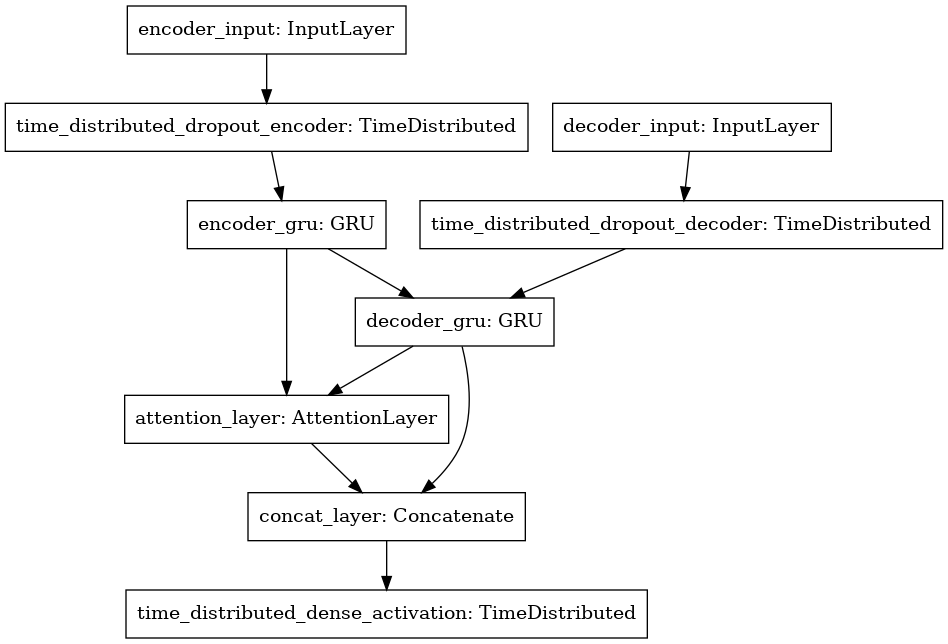
\includegraphics[width=1.1\textwidth]
        {model.png}
      }
    \caption{The Keras model behind the chatbot.}
    \label{fig:keras-model}
  \end{figure}
\end{center}

In this model, the encoder LSTM is fed one-hot encoded utterances one at a
time. Recall that the purpose of this step is to create a compact, internal
representation of the input utterance - a thought vector, so to speak. The
enoder LSTM outpts a list containing outputs from the encoder as well as the
internal encoder state. The decoder LSTM discards the LSTM output, but uses
the final hidden encoder state as its own initial state, so that the decoder
also has information about the input utterance. As input, the decoder layer
is fed the target sequence - that is, the response utterance. As a target for
output, the decoder is fed the same target sequence, but shifted to the right
by one. This is a training method which is known as teacher forcing
\cite{teacher-forcing}. It simply means that the network is taught to output
token $n$ in the utterance, given token $n-1$ as input. The alternative to
teacher forcing is to feed the decoder prediction back into the decoder output,
instead of always using the ground truth as the decoder input. However, not
using teacher forcing generally makes training slower and the model unstable.
\todo{I don't really understand this stuff thoroughly. Triple check solidness, elaborate more.}
\todo{Object oriented system. Explain LSTM nodes. Object oriented system. How we fit the model. Epochs, batches.}

\subsection*{Inference}

Once a model is trained, we can use it to generate responses to input
utterances. This is a separate phase from the training phase, which is usually
referred to as the inference phrase. We now provide a high-level description
of the inference phase used in this chatbot system.

\paragraph{}
When the system receives an input utterance from the user, we first run the
preprocessing step on the utterance to ensure it conforms to the same
specifications as the input data used while training. Then, this processed
input utterance is fed to the encoder, and the final hidden encoder state is
used as the initial state for the decoder, just as in the training phase. We
then run the decoder, using the special \emph{<BOS>} token as the input. This
yields the initial token of the response utterance. The system then feeds this
token back into the decoder, and uses it to generate the next token in the
utterance. At each step in this process, the system picks the most likely
token. This process halts when the special \emph{<EOS>} token is generated,
at which point the response utterance is returned to the user.
\todo{Might want to discuss the stated stored at each step, but I don't really know enough about that stuff to write about it.}

\paragraph{}
The inference system just described is a greedy decoding scheme, as the token
picked is always just the most likely token. However, this basic scheme does
not always yield the most likely \emph{utterance}. Future work might explore
alternative inference schemes based on algorithms such as beam search, which
seek to maximize the probability for the entire output utterance.

\subsection*{}

% Architecture \ Experimental Setup + Teacher forcing Future work: Bert/custom
% embeddings, embedding layer, bidirectional model, beam search

\section*{Related Work}
Multiple Norwegian chatbots already exist. However, these are usually systems
which first map the user query to a predefined intent, and then retrieve an
answer from a list of answers belonging to the intent. Such systems require a
fair amount of manual training, and lack the ability to independently formulate
an answer independently, based only on the question.  In this report, we
describe a generative chatbot which is based on an unsupervised model.

\section*{Results}

% Å analysere gjør du ved å redegjøre, forklare og vurdere funnene dine.
% Analysedelen av oppgaven blir ofte kalt resultater, slik som i
% IMRoD-modellen.  I kvantitative studier vil du kanskje i tillegg til å
% presentere funnene skriflig, bruke figurer og tabeller for å gi leseren en
% oversikt og innsikt i hva du har gjort.  I empirisk baserte studier vil
% analysene handle om å beskrive og tolke. Mange vil ofte drøfte enkeltfunnene
% i dette kapitlet og ta for seg mer overordnede funn i drøftingskapitlet.

\section*{Discussion / Evaluation}

% Du skal her drøfte resultatene dine og sette dem inn i en sammenheng. Å
% drøfte vil si å: sette ulike synspunkter, momenter, argumenter, faktorer og
% årsaker opp mot hverandre vurdere og sette dem opp mot hadily available, this
% is one of the primary challenges.  + Facebook Messenger data dump.  +
% Clarino: Tried, but restrictive licenses.  + Movie scripts. Copyright
% unclear.

% heavily biased dataset bad training data, not so much training data simple
% model

% heavily biased dataset
% bad training data, not so much training data
% simple model

\section*{Conclusion}

% Om avslutningen din skal være en konklusjon eller en oppsummering, avhenger
% av problemstillingen din. En konklusjon skal svare på problemstillingen, mens
% en oppsummering gjentar det viktigste fra oppgaven. Det er ikke uvanlig å
% velge en kombinasjon av de to, hvor du både oppsummerer oppgaven kort, men
% også svarer på problemstillingen.  Det er lurt å la avslutningen speile
% innledningen, ved å si hva du har gjort. Avslutningen bør også sette oppgaven
% din i et større perspektiv, og peke på hvilke muligheter du ser ut fra ditt
% prosjekt. Hvilke bidrag har din undersøke gitt til faget? Er det noe som
% burde blitt studert ytterligere? Slik tar du utgangspunkt i ditt eget
% prosjekt og peker på mulighet for oppfølging.

\todo{Conversation data in appendix.}

\printbibliography

\end{document}
